% Chapter 2


\chapter{Background} % Write in your own chapter title
\label{Chapter2}
\lhead{} % Write in your own chapter title to set the page header

\section{Interpretability in AI}

\subsection{Definition}

Over the past decade, the field of artificial intelligence (AI) has experienced rapid growth, becoming increasingly prevalent in automated decision-making processes across various sectors, both public and private. With the proliferation of machine learning systems, there is a growing need to understand and interpret the reasoning behind their decisions.

Interpretability in AI refers to the ability to understand and explain how machine learning models arrive at their conclusions \cite{intepretai}. As machine learning systems become more complex, understanding their decision-making processes becomes increasingly challenging. This lack of interpretability presents a fundamental obstacle to the widespread adoption of AI systems in critical domains.

The discussion surrounding the explainability of AI revolves around the study of how to comprehend the decisions made by machine learning systems and how to design systems whose decisions can be easily understood or interpreted. Strengthening interpretability, verifying the functionality of AI systems, and offering explanations for unexpected behaviors collectively builds trust and confidence in decision-making processes driven by AI.

\subsection{Importance of Interpretability}

In many aspects of society, there exists a fundamental expectation for the right to request an explanation for decisions, particularly when those decisions may have adverse consequences. This expectation extends across various domains, from employment discrimination cases to financial transactions and even military proceedings.

However, when decisions are made by machine learning systems, this expectation becomes more complex. Unlike human decision-makers, machine learning systems may lack the ability to provide explanations for their decisions, posing challenges in ensuring accountability and adherence to established standards.

For modern machine learning systems to integrate safely into existing institutions, especially in high-stakes settings, interpretability becomes essential.  In high-stakes applications such as automated credit scoring, medical diagnoses, hiring, and autonomous driving, the decisions made by these systems can have significant implications for individuals and society at large. Human operators must be able to understand and interpret the decisions made by these systems, allowing for accountability and trust in their outcomes.

In below subsections we discuss the problem of intepretability of AI in \textit{Computer Vision} (CV) and what are some methods used to address it along what are their limitations. 


\subsection{Interpretability in Computer Vision and Saliency Maps}

Interpretability in CV can refer to the ability to explain and understand how a model arrives at its predictions, especially in complex tasks such as image classification.

One popular approach to enhance interpretability in computer vision is the use of saliency maps \cite{saliency}. These maps visualize which areas of an image contribute most to a model's classification decision. For example, when analyzing an image of a German Shepherd classified as a dog, a saliency map may highlight features characteristic of dogs, such as a large muzzle, tail etc.

Figure \ref{fig: saliency_map} below illustrates examples of images alongside their corresponding saliency maps, demonstrating how saliency maps can provide insights into the decision-making process of machine learning models. 

\begin{figure}[htbp]
  \centering
  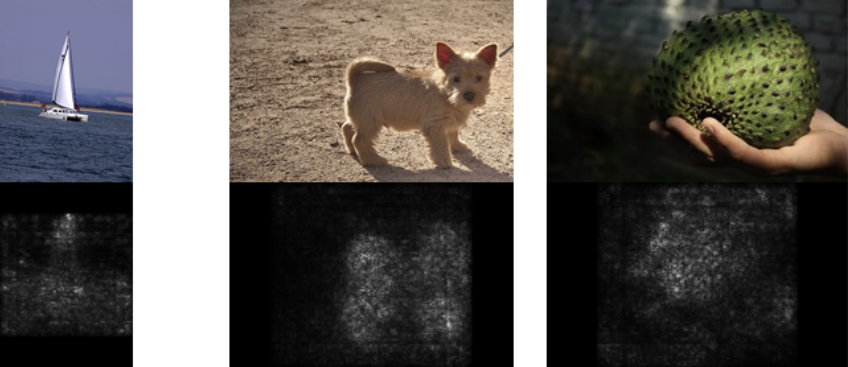
\includegraphics[width=\textwidth]{./Figures/saliency.png}
  \caption{Examples of images and their corresponding saliency maps indicating which parts of the images contribute most to how a machine learning system trained on a large set of images would classify them. Source: \cite{simonyan2014deep}}
  \label{fig: saliency_map}
\end{figure}

\subsection{Visualizing Model Components}

Another effective method for enhancing interpretability is to visualize how different components of a model relate to high-level concepts. For instance, in image classifiers, visualizations can show how different layers of the network detect lines, textures, and objects of increasing complexity.

Figure \ref{fig: layer_perspective} showcases examples of visualizations depicting what different layers of an image classification network "see," highlighting the progression from simple features to more complex objects.

\begin{figure}[htbp]
  \centering
  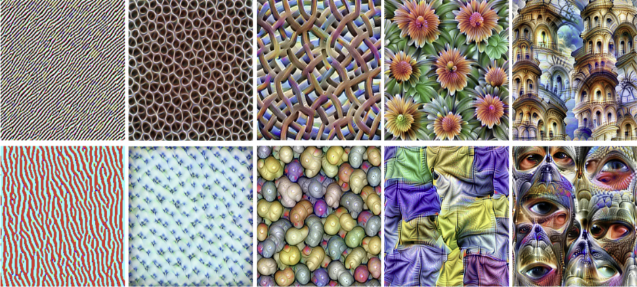
\includegraphics[width=\textwidth]{./Figures/layer_perspective.png}
  \caption{A visualization showing examples of what different layers of an image classification network “see.” The left-most column, depicting an early layer, is picking up lines; middle layers are detecting textures and patterns of increasing complexity; later layers, shown on the right, are looking for objects. Source: \cite{olah2017feature}}
  \label{fig: layer_perspective}
\end{figure}

\subsection{Limitations of Existing Methods}

Despite the effectiveness of saliency maps and visualizations, existing methods for enhancing interpretability have limitations. They often provide only a partial view of the system's decision-making process, lacking a comprehensive understanding of how data and learning algorithms interact during training. As a result, insights obtained from existing methods may be incomplete or require human supervision.


\section{Data-Driven Deep Learning and Model-Based Algorithms}
In the previous section, we discussed the limitations of current methods for achieving interpretability in AI systems. We explored the challenges posed by the increasing complexity of machine learning models and the difficulty in understanding how they reach conclusions. It turns out that to understand why this problem is prevalent, more so now than ever before, lies in the understanding of how traditionally problems in fields like signal processing, digital communications, and medical imaging etc were handled - termed as \textit{Model-Based} methods - vs the more popular approach \textit{Data-Driven} methods. We will explain the key differences between these two using a nice example found in \cite{LUIJTEN2023677}. 

\subsection{Model-Based Methods}

Consider the following general linear model:

\begin{equation}
    \mathbf{y} = \mathbf{A}\mathbf{x} + \mathbf{n} \label{eq:1}
\end{equation}

In this model:
\begin{itemize}
    \item $\mathbf{y}$ represents the observed signal or image, possibly corrupted by noise during acquisition or transmission.
    \item $\mathbf{A}$ is the measurement or feature matrix.
    \item $\mathbf{x}$ denotes the signal of interest (e.g., the clean or original image).
    \item $\mathbf{n}$ is the noise vector, which could result from sensor noise, environmental factors, or compression artifacts.
\end{itemize}

In many signal processing problems, including image denoising, this linear model serves as a basis \cite{elad2023image}.

Sometimes, the noise vector comprises a combination of sparse, high-variance components and dense, low-variance Gaussian noise, known as impulsive Gaussian Mixture Model (GMM) distributed noise (reference needed). We'll delve into this further when discussing matrix completion.

Our objective is to recover the clean or original image as accurately as possible.

By applying Bayes’ rule, we define the posterior probability of $\mathbf{x}$ given $\mathbf{y}$ as the product of the likelihood $p(\mathbf{y|x})$ and a prior $p(\mathbf{x})$, yielding:

\begin{equation}
    p(\mathbf{x|y}) = \frac{p(\mathbf{y|x})p(\mathbf{x})}{p(\mathbf{y})} \label{eq:2}
\end{equation}

From Equation~\eqref{eq:2}, a maximum a posteriori (MAP) estimator for Equation~\eqref{eq:1} is derived:

\begin{equation}
    \hat{\mathbf{x}}_{\text{MAP}} = \arg\max_{\mathbf{x}} p(\mathbf{x|y}) = \arg\max_{\mathbf{x}} p(\mathbf{y|x})p(\mathbf{x}) \label{eq:4}
\end{equation}

This estimator provides the most likely estimate according to the posterior distribution. Assuming an additive Gaussian white noise vector $\mathbf{n}$ in Equation~\eqref{eq:1}, i.e., $\mathbf{y} \sim \mathcal{N}(\mathbf{Ax}|\sigma^2_n\mathbf{I})$, the MAP estimator can be expressed as:

\begin{equation}
    \hat{\mathbf{x}} = \arg\min_{\mathbf{x}} \|\mathbf{y} - \mathbf{Ax}\|_2^2 + \lambda \log p(\mathbf{x}) \label{eq:5}
\end{equation}

Here, $\lambda$ is a scalar regularization parameter.


Evidently, the MAP estimator takes allows us to incorporate and exploit prior information on \( \mathbf{x} \), should this be available. Conversely, if \( \mathbf{x} \) is assumed to be deterministic but unknown, we get the maximum likelihood (ML) estimator. The ML estimator thus assigns equal likelihood to each \( \mathbf{x} \) in the absence of measurements. As such, this simplifies to
\begin{equation}
    \hat{\mathbf{x}}_{\text{ML}} = \arg\max_\mathbf{x} p(\mathbf{y}|\mathbf{x}) \label{eq:6}
\end{equation}

Traditional signal processing is predominantly governed by algorithms grounded in simple mathematical models that are built from domain expertise. This knowledge may stem from statistical models based on measurements and an understanding of the underlying physics or from a predetermined deterministic representation of the specific problem under consideration. These model-based methods conduct inference based on the known model linking the available observations with the desired information. While model-based methods do not rely on data to learn their mapping, data are often utilized to estimate a small number of parameters.

Classical statistical models hinge on simplifying assumptions (e.g., linearity, Gaussian distribution, and independent noises as those found in \textit{OLS} \cite{albert_ols_review}) that render inference manageable, easily comprehensible, and computationally efficient. However, these simple models frequently fail in capturing the subtleties of high-dimensional complex data and dynamic variations. Moreover, if any of these assumptions are violated, the model fails.

% Data-driven approaches aim to overcome the challenges of accurate modeling by learning the likelihood function, the prior, the entire posterior, or a direct end-to-end mapping (replacing the complete MAP estimator) from data. We will detail on these methods in the following section. 

\subsection{Data-Driven Learning}

The remarkable success of deep learning has fostered a widespread adoption of data-driven methodologies. It has become increasingly common to replace simple principled models with purely data-driven pipelines, trained using vast labeled datasets, especially given the ubiquitous availability of data. Fully data-driven methods aim to learn the optimal parameters $\theta$ of a generic parameterized mapping $f_{\theta}: Y \rightarrow X$, from training data $\mathcal{D}$. In the context of deep learning, the mapping function $f_{\theta}(\cdot)$ typically represents a deep neural network.

Learning can be formulated as a probabilistic inference problem, where optimized parameter settings for a fixed network architecture are inferred from the dataset $\mathcal{D}$. This inference is based on a posterior distribution over the parameters $\theta$:
\begin{equation}
p(\theta|\mathcal{D}) = \frac{p(\mathcal{D}|\theta)p(\theta)}{p(\mathcal{D})} \quad \label{eq:7}
\end{equation}

Here, $p(\theta)$ denotes a prior distribution over the parameters. Often, the prior $p(\theta)$ is fully factorized, assuming independence among parameters, to manage the learning problem in deep networks with millions of parameters.

Many DL applications rely on Maximum A Posteriori (MAP) estimation to find the set of parameters that minimize the negative log posterior:
\begin{equation}
\theta^* = \arg\max_{\theta} p(\theta|\mathcal{D}) = \arg\max_{\theta} \log p(\mathcal{D}|\theta) + \log p(\theta) 
\end{equation}
\begin{equation}
= \arg\min_{\theta} \left\{ -\log p(\mathcal{D}|\theta) - \log p(\theta) \right\}
\end{equation}


For pairs of measurement (input) signals and corresponding output training data $(\mathbf{y}_i, \mathbf{x}_i) \in \mathcal{D}$, common forms of $p(\mathbf{x}|f_{\theta}(\mathbf{y}), \theta)$ include Gaussian whose MLE estimate results in minimizing mean squared error. After training, i.e., inferring parameter settings, the network can be used to perform MAP inference to retrieve $\mathbf{x}$ from new input measurements $\mathbf{y}$:
\begin{equation}
    \hat{\mathbf{x}} = \arg\max_{\mathbf{x}} p(\mathbf{x}|f_{\theta}(\cdot), \theta) 
\end{equation}

The neural network directly models the parameters of the posterior without factoring it into a likelihood and prior term as model-based MAP inference does. Typical deep neural network parameterizations $f_u(\cdot)$ are therefore model-agnostic, as they disregard the structure of the measurement/likelihood model and prior, offering a high degree of flexibility to fit many data distributions and problems. However, many such parameterizations exploit specific symmetries in the expected input data. For instance, convolutional neural networks exploit the spatial shift-invariant structure of many image classification/regression problems through shift-equivariant convolutional layers. Similarly, in applications where the input is temporally correlated, such as time series analysis, recurrent neural networks (RNN) are employed.

The advantages of data-driven methods over model-based approaches are twofold: Firstly, purely data-driven techniques do not rely on analytical approximations and can operate in scenarios where analytical models are not known. Secondly, for complex systems, data-driven algorithms can recover features from observed data necessary for inference, which may be difficult to achieve analytically even with perfectly known complex models. However, the computational burden of training and utilizing highly parameterized DNNs, along with the requirement for massive datasets to train such DNNs for learning a desirable mapping, may present significant drawbacks in various signal processing, communications, and control applications. This is particularly pertinent for hardware-limited devices, such as mobile phones, unmanned aerial vehicles, and Internet-of-Things (IoT) systems, which are often constrained in their ability to utilize highly parameterized DNNs and require adaptation to dynamic conditions.

It's worth noting why the term “black box,” often used in this context, is not entirely accurate in describing why deep neural networks are challenging to understand. Machine learning researchers comprehend how the mathematical operations underlying these systems work, and it's straightforward to examine the parameter values that constitute the model. The challenge lies in understanding how millions (or even billions) of number values relate to the concepts of interest, such as why a machine learning model may misclassify a cat as a dog. In other words, interpreting deep neural networks requires both understanding which high-level features in the data—such as a specific part of an image or a particular sequence of words—affect a model’s predictions and why a model associates certain high-level features with a corresponding prediction—that is, how deep neural networks “reason” about data. Consequently, deep learning does not yet offer the interpretability, flexibility, versatility, and reliability of model-based methods. For e.g , a recent paper  \cite{bai2021attentions} has shown why the main machinery of \textit{transformers} - attention mechanism - might not be performing in the way its expected.


\subsection{Model - Based Deep Learning}
In many applications, such as those which drive new material discovery, constitutive models are sought that have three characteristics: (1) the ability to be derived in automatic fashion with (2) high accuracy and (3) an interpretable nature \cite{BOMARITO2021106557}. As discussed, traditionally developed models are usually interpretable but sacrifice development time and accuracy. Purely data-driven approaches are usually fast and accurate but lack interpretability.

Model-based DL aims at imposing much more structure to the network architectures and parameterizations of $f_\mathbf{\theta}(\cdot)$. Where standard deep networks aim at fitting a broad class of problems, model-based DL offers architectures that are highly tailored to specific inference problems given in equations \eqref{eq:1} and \eqref{eq:4}; that is, they are aware of the model and structure of the problem. This promises to relax challenges related to generalization, robustness, and interpretability in DL. It often also enables the design of smaller (but more specialized) networks with a lower computational and memory footprint.

To derive a model-based DL method, one can start by deriving a MAP estimator for $\mathbf{x}$ from the model, including assumptions on likelihood models $p(\mathbf{y|x})$ and priors $p(\mathbf{x})$. Generally, such estimators come in two forms: analytic (direct) and iterative solutions. The solution structure dictates the neural network architecture. One then has to select which parts of the original model-based graph are to be replaced by learnable functions.

One of the first examples of model-based DL is the learned iterative-shrinkage and thresholding algorithm (LISTA), proposed by Gregor and LeCun \cite{lista} as an unfolding of two popular iterative solvers ISTA and FISTA \cite{ista}. As the name suggests, $\mathbf{f_{theta}}(\cdot)$ is based on an iterative solution, specifically to the MAP sparse coding problem: $\arg\max_x p(\mathbf{y|x})p(\mathbf{x})$, with $\mathbf{x} \sim \text{Laplace}(0, b\mathbf{I})$, where $b$ is a scale parameter, and $\mathbf{y|x} \sim \mathcal{N}(\mathbf{Ax}, \sigma^2\mathbf{I})$. This iterative solution consists of two alternating steps: (i) a gradient step on $\mathbf{x}$ to maximize the log-likelihood of $\log p(\mathbf{y|x})$, and (ii) a proximal step that moves the intermediate solution for $\mathbf{x}$ toward higher log-likelihood under the prior distribution $\log p(\mathbf{x})$. The model-based DL method LISTA unfolds or unrolls a limited number of algorithm iterations to form a feed-forward neural network, learning the parameters of the gradient step and the proximal step end-to-end from training examples $(\mathbf{y_i}, \mathbf{x_i}) \in \mathcal{D}$, without knowledge of the underlying distribution of these parameters. Moreover, LISTA and its unfolded variants such as LISTA-CPSS, TiLISTA and ALISTA show faster convergence and lower loss in compressive sensing as shown in below Figure \ref{fig: lista}.  

\begin{figure}[htbp]
  \centering
  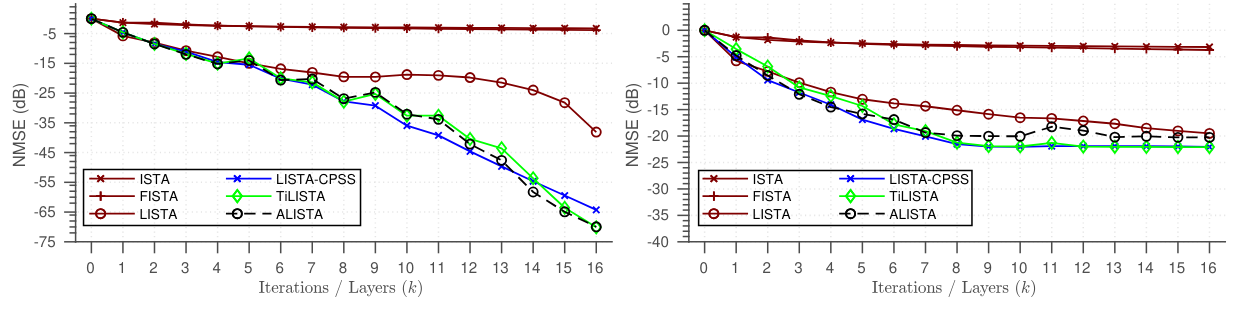
\includegraphics[width=\textwidth]{./Figures/lista.png}
  \caption{L2O optimizers (LISTA, LISTA-CPSS, TiLISTA and ALISTA) converge much faster than the two popular iterative solvers (ISTA, FISTA). Left: noiseless case. Right: noisy case (SNR = 20). Source: \cite{liu2019alista}}
  \label{fig: lista}
\end{figure}

Model-Based DL is also deeply linked with the idea of \textit{L20} \cite{chen2022learning}, an emerging approach that leverages machine learning to develop optimization methods, aiming at reducing the laborious iterations of hand engineering. It automates the design of an optimization method based on its performance on a set of training problems. When it comes to problems where the target solutions are difficult to obtain, such as nonconvex optimization and inverse-problem applications, the solution of a well-trained L2O method can have better qualities than those of classic methods. However, it's imperative to note that the L2O or Model-Based DL is suitable for repeatedly solving a particular optimization problem over a specific distribution of data, while it typically fails on out-of-distribution problems. Thus its practicality depends on the type of target optimization, the chosen architecture of the method to learn, and the training procedure. To conclude the following Figure \ref{fig: overview} nicely depicts each of the three methods, i) Model-Based, ii) Data-Driven Deep Learning and finally iii) Model-Based Deep Learning. 

\begin{figure}[htbp]
  \centering
  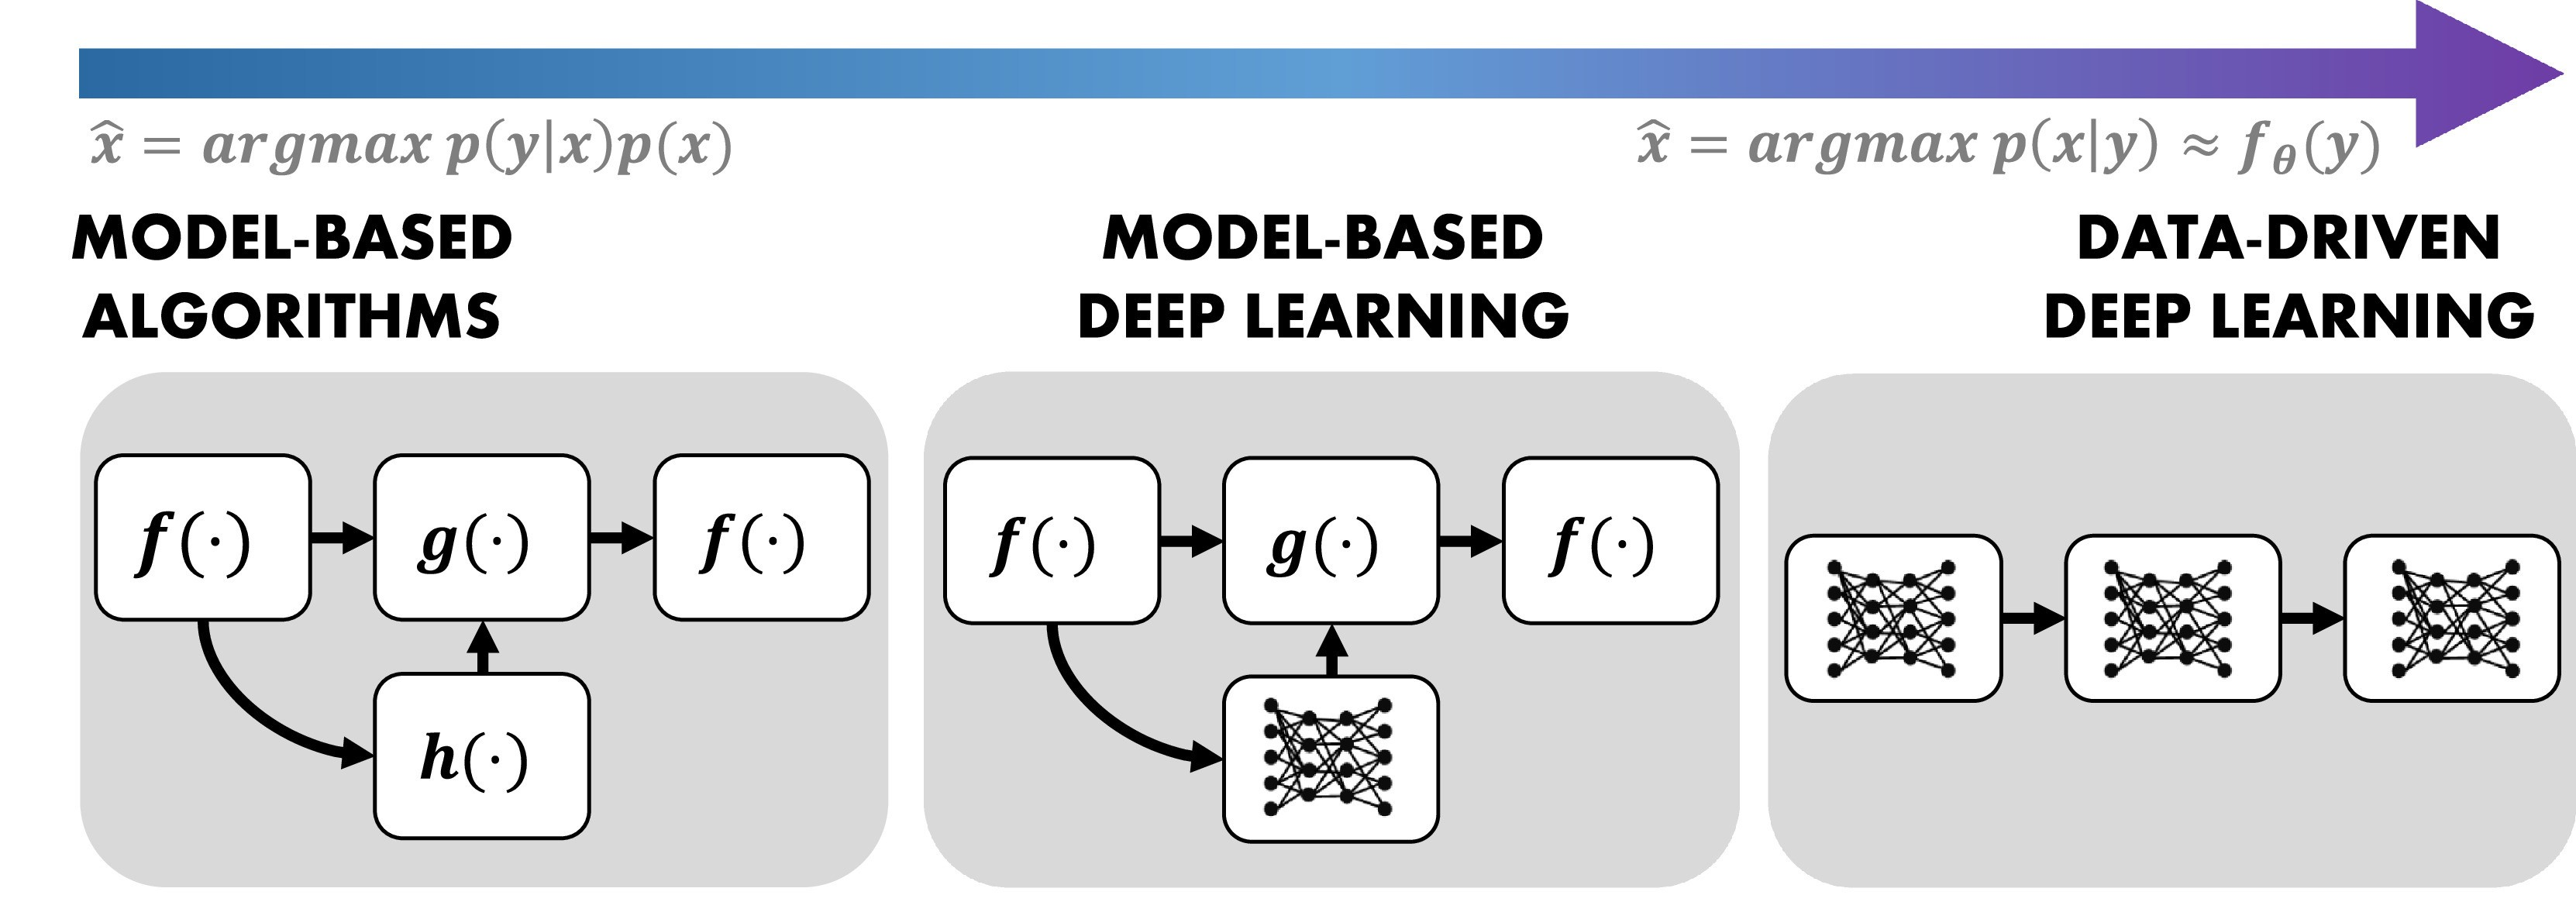
\includegraphics[width=\textwidth]{Figures/overview.jpg}
  \caption{Schematic overview of model-based and deep learning. Source: \cite{LUIJTEN2023677}}
  \label{fig: overview}
\end{figure}


\section{Matrix Completion}

\subsection{Problem and Motivation}

During the past few years, matrix completion (MC) has received increasing interest worldwide for its unique property and numerous applications in traffic sensing \cite{traffic_sensing}, integrated radar and communications \cite{radar_communications}, image inpainting (more on it later) \cite{image_inpainting}, recommendation systems with the most common being the \textit{Netflix Prize} problem \cite{jackson2017netflix}, and so on. Subsequent to compressed sensing (CS), MC is another significant technology utilizing sparse property to process data. Sparsity, in CS, means that the signal of interest contains lots of zero elements in a specific domain. However, in MC, it indicates that the singular value vector of the original matrix is sparse. In other words, the matrix is \textit{low-rank}.

MC is able to restore the original signal $X$ from a fragmentary signal $X_{\Omega}$ (or called the undersampled/incomplete signal), where $\Omega$ is a subset containing $2D$ coordinates of sampled entries. The undersampled signal $X_{\Omega}$ can be expressed as:
\begin{equation}
    X_{\Omega} = H_{\Omega} \odot X + N \label{eq: 8}
\end{equation}

\[
H(i, j) = 
\begin{cases}
1 & \text{if } (i, j) \in \Omega \\
0 & \text{otherwise}
\end{cases}
\]
where all variables belong to $\mathbb{R}^{n \times m}$, $\odot$ is the element wise multiplication (Hadamard) operator, $H_{\Omega}$ and $N$ are the sampling matrix and noise matrix, respectively. Note that $H_{\Omega}$ is a binary matrix, which are drawn from a random uniform distribution to ensure at least one $1$-element in each row and column. Furthermore, it is assumed that the original signal $X$ has the low-rank or approximately low-rank property.

Low-rank property of signals is ubiquitous in real-world applications. For instance, data collection of wireless sensor networks (WSNs) \cite{wireless_sensor}.Spatio-temporal signals are time series collected over a certain spatial range \cite{spatial}. In many cases, the collected spatio-temporal data is incomplete because of the limited power supply or malfunctions \cite{missing_node}. Hence, recovery of spatio-temporal signals from incomplete data is a critical issue in WSNs.The main information conveyed by the measurement matrix is dominated by some largest singular values, whereas the remaining smallest singular values can be taken as zero without losing major information. Thus, the measurement matrix has an approximately low-rank structure.

It is proposed to utilize rank minimization problem to restore the original signal $X$. The MC problem under the noise-free environment is formulated as:
\begin{equation}
    \min_{M} \text{rank}(M), \quad \text{s.t.} \quad M_{\Omega} = X_{\Omega} \label{eq: 9}
\end{equation}

where $M \in \mathbb{R}^{m \times n}$, $X_{\Omega} = H_{\Omega} \odot X$, and $M_{\Omega}$ denotes the projection on $\Omega$. When the sampled signal is corrupted by noise, there is a need to constrain the noise level within an appropriate range. As a result, the MC problem can be expressed as:
\begin{equation}
    \min_{M} \text{rank}(M), \quad \text{s.t.} \quad \|M_{\Omega} - X_{\Omega}\|_F \leq \delta \label{eq: 10}
\end{equation}

where $X_{\Omega}$ is defined by Equation \ref{eq: 8}, $\|\cdot\|_F$ denotes the Frobenius norm of a matrix, and $\delta > 0$ is a tolerance parameter that limits the fitting error.

Unfortunately, the rank minimization problem is NP-hard since all algorithms for exactly solving \ref{eq: 9} and \ref{eq: 10} are doubly exponential in dimension $\max(m, n)$ in both theory and practice. This is why all state-of-the-art algorithms attempt to solve the \textit{approximate} problem of rank minimization. This is done by replacing rank minimization problem with a \textit{nuclear norm} minimization (NNM) problem. \cite{fazel2002matrix} proved that the nuclear norm is the convex envelope of rank, which turns out to be a convex relaxation and in turn enables one to efficiently solve the issue of rank minimization in MC. This convex relaxation is akin to the relaxation of $\ell_0$ minimization to $\ell_1$ minimization in CS \cite{candes2008introduction}.

Subsequently, Cand\`es and Recht proposed to solve the rank minimization problem in \ref{eq: 9} by the nuclear norm minimization problem, given as:
\begin{equation}
    \min_{M} \|M\|_*, \quad \text{s.t.} \quad M_{\Omega} = X_{\Omega} \label{eq: 11}
\end{equation}

where $\|\cdot\|_*$ is the nuclear norm of a matrix defined as the sum of singular values$ \| M \|_* = \sum_{i=1}^{\min\{m,n\}} \sigma_i(M)$.


\subsection{MC Formulations}
Various MC methodologies have been developed from different perspectives, with pros and cons. To facilitate readers, we present a brief summary of several well-known MC algorithms in Table \ref{tab:mc_algorithms}.

\begin{table}[H]
\centering
\caption{Summary of Matrix Completion Algorithms}
\label{tab:mc_algorithms}
\begin{tabular}{@{}lll@{}}
\toprule
NNM & Normal Situation & Outlier Situation \\ \midrule
Nuclear norm relaxation & Matrix factorization & $\ell_{p}$ norm minimization \\
Semidefinite programming & Minimum Rank Approximation & Adaptive outlier pursuing\\
Robust PCA &  &  \\ \bottomrule
\end{tabular}
\end{table}

We will only discuss methods for i) NNM, ii) matrix factorization and iii) $\ell_p$-norm minimization in this paper. RPCA will be briefly mentioned but later discarded due to its limitations.

\subsubsection{Nuclear Norm Minimization}
Based on NNM, the singular value thresholding (SVT) \cite{SVT} approach proposed to use a proximal objective of nuclear norm minimization is given as:
\[
\min_{M} \tau \|M\|_* + \frac{1}{2} \|M\|_F^2, \quad \text{s.t.} \quad M_{\Omega} = X_{\Omega} 
\]
where $\tau \geq 0$. Note that the parameter $\tau$ provides a tradeoff between the convex-non smooth nuclear norm and convex, smooth Frobenius norm. Such minimization problems that can be broken down that can be decomposed in this way are often solved by setting up the lagrangian:
\begin{equation}
    L(M, Y) = \tau \|M\|_* + \frac{1}{2} \|M\|_F^2 + \langle Y, M_{\Omega} - X_{\Omega} \rangle. \label{eq: 12}
\end{equation}

where $Y \in \mathbb{R}^{n \times m}$ is the lagrange multiplier. 
To solve \ref{eq: 12}, Cai et al. \cite{cai2010singular} introduced a proximity operator associated with the nuclear norm. In particular, a soft-thresholding operator $D_{\tau}$ is introduced, which is defined as:
\begin{equation}
    D_{\tau}(Y) := U D_{\tau}(S) V^T, \quad D_{\tau}(S) = \text{diag}\{(\sigma_i - \tau)^+\}_{i=1}^r,
\end{equation}

where $r$ is the rank of $Y$, $Y = USV^T$ is the singular value decomposition (SVD) of $Y$ with $S = \text{diag}\{\sigma_i\}_{i=1}^r$, $U \in \mathbb{R}^{n \times r}$ and $V \in \mathbb{R}^{m \times r}$ being orthonormal matrices, and $(t)^+ = \max(0, t)$. Notably, each iteration in solving \ref{eq: 12} requires calculating the SVD of $Y$ and then obtaining $D_{\tau}(Y)$. This will be one of the main points we take into consideration later on when devising a model to unfold. 

\subsubsection{Robust PCA}
Lin et al. \cite{rpca} considered the MC problem as a special case of robust principal component analysis (PCA) problem and formulated it as:
\begin{equation}
    \min_{M} \|M\|_*, \quad \text{s.t.} \quad M + S = X_{\Omega}, \quad S_{\Omega} = 0 \label{eq: 13}
\end{equation}

where $S \in \mathbb{R}^{n \times m}$ is a sparse matrix. The inexact augmented Lagrange multipliers (IALM) \cite{rpca} solves the augmented Lagrange version of the above to obtain the result $M$. However, this approach does not consider the noisy environment due to $S_{\Omega} = 0$, thereby prohibiting its applications.

Based on the weighted nuclear norm \cite{wnnm}, the variant of robust PCA for MC was devised in \cite{wnnm}, which is formulated as:
\begin{equation}
    \min_{M} \|M\|_{w,*}, \quad \text{s.t.} \quad M + S = X_{\Omega}, \quad S_{\Omega} = 0 \label{eq: 14}
\end{equation}

It should be noticed that although the standard robust PCA for low-rank matrix recovery is able to process impulsive noise, the robust PCA for MC in \ref{eq: 13} and \ref{eq: 14} is not robust against impulsive noise. The standard robust PCA is formulated as:
\begin{equation}
    \min_{L,S} \|L\|_* + \lambda \|S\|_1, \quad \text{s.t.} \quad L + S = D \label{eq: 15}
\end{equation}

where $L \in \mathbb{R}^{n \times m}$ is the target matrix with low-rank property, $\lambda > 0$. Interestingly, $S$ in the constraint of \ref{eq: 15} can be taken as impulsive noise added to $L$. Accordingly, its sparse property can be characterized by the $\ell_1$-norm. Therefore, the standard robust PCA is robust against impulsive noise whereas its variant for tackling the MC problem does not retain this robustness. Actually, if the sampled entries in \ref{eq: 13} are corrupted by additive noise, the noise term cannot be suppressed due to $S_{\Omega} = 0$. This is why the robust PCA for MC has a bad performance in the case of noise, not to mention impulsive noise.

Although the MC approaches are capable of offering superior performance by tailoring the nuclear norm minimization criterion, they suffer from low computational efficiency and limited scalability in big-scale data. To circumvent this issue, the \textit{matrix factorization} (MF) \cite{matrix_factorization} was proposed to solve the MC problem without SVD. The basic idea behind the MF methodology is to utilize two low-rank matrices ($U \in \mathbb{R}^{n \times r}$ and $V \in \mathbb{R}^{m \times r}$) Denoting $M = UV$, yields the following optimization problem:
\[
\min_U \min_V \| (UV^T)_{\Omega} - X_{\Omega} \|_F^2
\].

We discuss how these types of structures are solved later on. 

\subsubsection{$\ell_p$-Norm Minimization}
Consider the case for impulsive noise which usually corrupts the received data in real-world applications. The $\ell_2$-norm cannot exactly characterize the behaviors of both impulsive and Gaussian noises. It is easy to understand this statement because the $\ell_2$-norm may seriously amplify the power of impulsive noise, which is much larger than the power of Gaussian noise. This thereby motivates one to exploit other metrics for the impulsive noise scenario. For a matrix $R$, $\ell_p$-norm is defined as:
\[
\|R\|_{p} = \left( \sum_{i,j} |R_{i,j}|^p \right)^{\frac{1}{p}}
\]
where $[R]_{i,j}$ is the element of $R$.

$\ell_p$-norm with $0 < p < 2$ is able to resist outlier and thereby has been widely adopted to handle the impulsive noise. This is because, roughly speaking, $|[R]_{i,j}|^p$ measures the level of our dislikes of $R_{i,j}$. If $|R_{i,j}|^p$ is very small, it does not affect the recovery performance. If $|R_{i,j}|^p$ becomes large, however, it is indicated that we have to handle strong dislikes for these large residuals. Dislikes correspond to the values we need to minimize. For instance, compared with $|R_{i,j}|$, $|R_{i,j}|^2$ magnifies residuals, especially the residuals associated with outliers. In other words, to minimize the total residual, $\ell_p$-norm ($0 < p < 2$) pays more attention to minimize large residuals, i.e., outliers. Consequently, $\ell_p$-norm ($p = 1$) has a better performance than $\ell_2$-norm.

The $\ell_p$-regression ($\ell_p$-reg) algorithm \cite{lp_reg} combines the MF technique and $\ell_p$-norm to solve the MC problem, which is formulated as:
\[
\min_{U,V} {\|(UV^T)_{\Omega} - X_{\Omega}\|}_{p}^{p}, \quad \text{s.t.} \quad 0 < p < 2
\]
Note that if $p = 2$, we reduce the problem to a least square solution. Details skipped but we employ the Iterative Reweighted Least Squares Algorithm (IRLS) \cite{irls} for $1 < p < 2$. 

\subsection{Algorithms}
Numerous algorithms can be employed to solve the MC problems. In this section, we will review only one main technique of optimization - Alternative Direction Method of Multiplier (ADMM), which comes under \textit{non-gradient} approaches. Although there exists several others as shown in the Table below, the ones we discuss are relevant mostly to the algorithms/models we propose or compare our performance to. Moreover, Block Coardinate Descent (BCD) is similar to ADMM, one being an unconstrained optimization problem while the other being a constrained optimization problem.

\begin{table}[htbp]
\centering
\caption{A Summary of Optimization Methods}
\label{tab:optimization}
\begin{tabular}{@{}lll@{}}
\toprule
\multicolumn{1}{c}{\textbf{Gradient}} & \multicolumn{1}{c}{\textbf{Non-gradient}} \\ \midrule
GD &  BCD\\
APG  &ADMM  \\
BI  &  \\ \bottomrule
\end{tabular}
\end{table}

\subsubsection{Alternative Direction Method of Multiplier}

For constrained large-scale optimization problems, Gabay and Mercier \cite{ADMM} firstly introduced ADMM to tackle it.  According to the principle of ADMM, the constrained problem to be optimized can be expressed as
\begin{equation}
    \min_{X,Z} F(X) + G(Z) \quad \text{s.t.} \quad AX + BZ = C
    \label{eq: 16}
\end{equation}

where $F(X)$ and $G(Z)$ are convex, $X \in \mathbb{R}^{m \times r}$, $Z \in \mathbb{R}^{n \times r}$, $A \in \mathbb{R}^{p \times m}$, $B \in \mathbb{R}^{p \times n}$, and $C \in \mathbb{R}^{p \times r}$. The ADMM firstly converts \ref{eq: 16} to not only the Lagrangian but \textit{augmented} Lagrangian. 
\[
L_{\delta}(X, Y, Z) = F(X) + G(Z) + Y^T (AX + BZ - C) + \frac{\delta}{2} \|AX + BZ - C\|_F^2
\]

where $\delta > 0$. Then, the BCD approach is employed to optimize $X$, $Y$, and $Z$ separately. Algorithm \ref{algo: 1} summarizes the ADMM approach.

Notice how compared to the lagrangian we set up in \ref{eq: 12}, we have an extra term 'augmented' to the objective function $\frac{\delta}{2} \|AX + BZ - C\|_F^2$ which acts like the usual regularization and enforcement of the constraints we see in typical linear or logistic regression. 

\begin{algorithm}
  \caption{ADMM}
  \begin{algorithmic}[1]
    \State \textbf{Input:} Maximum iteration $N$, $X_0, Z_0$ and $\delta$
    \For{$k = 0, 1, ..., N$}
      \State $X_{k+1} = \text{arg} \min_{X_k} L_{\delta}(X_k, Y_k, Z_k)$
      \State $Z_{k+1} = \text{arg} \min_{Z_k} L_{\delta}(X_{k+1}, Y_k, Z_k)$
      \State $Y_{k+1} = Y_k + \delta(AX_{k+1} + BZ_{k+1} - C)$
    \EndFor
    \State \textbf{Output:} $X_{k+1}, Z_{k+1}$
  \end{algorithmic}
  \label{algo: 1}
\end{algorithm}

Further, notice that ADMM carries out \textit{dual ascent} update for the lagrange multuplier $Y$. This is because, the augmented Lagrangian method seeks a saddle point of $X$ and $Z$ by alternating between minimizing with respect to the primal variable $X$ and $Z$ and taking one step of gradient ascent to increase $X$ using the dual variable $Y$ \cite{Wright-Ma-2022}. 

The rest of the process is similar to that of BCD i.e. finding the optimal estimates of the parameters in a distributed manner, which significantly enhances the computational efficiency. The main principle behind the BCD and consequently ADMM algorithm is to optimize one parameter set while keeping other parameter sets unchanged at one time.

\section{Model-Based Deep Learning and Matrix Completion}

Despite the usefulness of this approach, it has rarely been employed to solve matrix completion problems that are pertinent in signal processing, wireless sensor networks, recommendation systems, and other domains. From what we have seen, ADMM-Net \cite{admm-net} and DMFC-Net\cite{ma2022deep} are the only ones who have applied this method for such problems and both have shown impressive results. Recently, there has also been an interest in reconstructing images and other forms of data that have been corrupted with impulsive GMM noise, but all of these have proposed iterative solutions that are subject to the aforementioned problems. Deep unfolding, however, has the potential to set a new benchmark for results in matrix completion problems, as indicated by its application in other domains. In the following section, we propose our idea and how it has the potential to perform better in terms of inference and accuracy when compared to the state of the art algorithms.



% \begin{thebibliography}{9}
% \bibitem{candes2010power}
% Candès, E.J., and Tao, T. (2010). The Power of Convex Relaxation: Near-Optimal Matrix Completion. \textit{IEEE Trans. Inf. Theory}, 56(5), 2053–2080.
% \bibitem{cai2010singular}
% Cai, J.F., Candès, E.J., and Shen, Z. (2010). A Singular Value Thresholding Algorithm for Matrix Completion. \textit{SIAM J. Optim.}, 20(4), 1956–1982.
% \bibitem{recht2010guaranteed}
% Recht, B., Fazel, M., and Parrilo, P.A. (2010). Guaranteed Minimum-Rank Solutions of Linear Matrix Equations via Nuclear Norm Minimization. \textit{SIAM Rev.}, 52(3), 471–501.
% \bibitem{jiang2019nonconvex}
% Jiang, H., Lu, Z., Lin, Z., and Zhang, C. (2019). Nonconvex Matrix Factorization from Rank-One Measurements. \textit{SIAM J. Optim.}, 29(1), 693–721.
% \bibitem{candes2011robust}
% Candès, E.J., Li, X., Ma, Y., and Wright, J. (2011). Robust Principal Component Analysis? \textit{J. ACM}, 58(3), Article 11, 37 pages.
% \bibitem{lin2010augmented}
% Lin, Z., Chen, M., and Ma, Y. (2010). The Augmented Lagrange Multiplier Method for Exact Recovery of Corrupted Low-Rank Matrices. \textit{arXiv preprint arXiv:1009.5055}.
% \bibitem{chen2011robust}
% Chen, Y., and Wiesel, A. (2011). Robust subspace recovery by weighted nuclear norm minimization. \textit{IEEE Trans. Inf. Theory}, 57(6), 3515–3529.
% \end{thebibliography}
